\section{Preprocessing}

\subsection{Raw Data}
All provided data are in the \ac{NIfTI} format, first these are need to be understood and parsed. This format stores the raw output of the \ac{MRI} record, and additionally an affine transformation matrix used for aligning different spaces.

\subsubsection{Available Data}
The following data will be preprocessed and read, even if not all of them are going to be used later on it helps providing the largest possible flexibility.

\begin{table}[H]
\centering
\begin{tabular}{|l|l|c|c|l|l|}
\hline
\textbf{Data} & \textbf{Shape} & \textbf{Range} & \textbf{Type} & \textbf{Space} & \textbf{Reference} \\ \hline
\ac{dMRI} & (118, 118, 60, 74) & $[0,4096]$ & uint & diffusion & diffusion \\ \hline
Diffusion \ac{FA} & (118, 118, 60) & $[0,~2]$ & float & diffusion & diffusion\_fa \\ \hline
Diffusion \ac{MD} & (118, 118, 60) & $[0,~0.01]$ & float & diffusion & diffusion\_md \\ \hline
Diffusion \ac{RD} & (118, 118, 60) & $[0,~0.01]$ & float & diffusion & diffusion\_rd \\ \hline
T1 & (208, 256, 256) & $[0,~1000]$ & float & t1 & t1 \\ \hline
T1/T2 & (208, 256, 256) & $[0,1]$ & float & d\_aligned & t1t2 \\ \hline
Cortical Targets & (118, 118, 60, 14) & $\{0,1\}$ & bool & diffusion & targets \\ \hline
Relative Connectivity & (118, 118, 60, 14) & $[0,1]$ & float & diffusion & connectivity \\ \hline
Streamline Image & (118, 118, 60, 14) & $[0,5000]$ & uint & diffusion & streamline \\ \hline
\ac{ROI} Mask (Basal Ganglia) & (118, 118, 60, 2) & $\{0,1\}$ & bool & diffusion & mask\_basal \& roi \\ \hline
Brain Mask & (208, 256, 256) & $\{0,1\}$ & bool & t1 & mask\_brain \\ \hline
Basal Ganglia Segmentation & (208, 256, 256) & $[0, 58]$ & uint & t1 & basal\_seg \\ \hline
\end{tabular}
\caption{Raw Datapoint}
\label{tab:datas1}
\end{table}

\subsubsection{Brain Mask}
The provided dataset did not apply the brain masks for the T1 images out of the box so it can be done with a simple element wise multiplication of the T1 image and T1 mask.

\subsubsection{Registration}
The process of aligning different records into the same native space is called "registration". The provided dataset comes with with 2 (3) different spaces, earlier referenced to as t1 and diffusion (and d\_aligned). Most of the data are in diffusion space, thus it is logical to register the rest into the same space. After manual inspection, only 15 datapoints required registration. Out of which 3 only required a tiny translation, and the rest 12 needed a complete affine registration.\par

The image T1/T2 is the odd one out, as it is inherently in a different space from diffusion (due to them being different resolution). But they are aligned into diffusion space. Although they do not need to be registered, this has to be taken into account later on.

\subsubsection{Normalization}
The process of warping each brain into a common space is called "normalization". Applying the \ac{FNIRT} warp fields are more or less straight forward, as two warp fields are provided, one for the diffusion space and one for the T1 space. Note that this process inherently contains the benefits of registration, as it is aligning the different images into a common space. This also paves the direction of future experiments, as it opens the door to working in either native and normalized space.\par

The only encountered obstacle was with the T1/T2 image. As it is aligned in diffusion space, but \ac{FNIRT} convention ignores the affine transformation of the \ac{NIfTI} format, thus making it's registration useless as the raw data of the t1t2 has nothing to do with the raw diffusion data (due to them being different resolution). The solution is to apply an affine matrix to t1t2's raw data which transforms it into t1's raw data space, after which the t1's \ac{FNIRT} warp field can be applied to the t1t2 image. This affine transformation matrix can be easily calculated from the already given matrices. Let $A$ denote T1/T2's affine matrix and $B$ denote T1's affine matrix (after registration), thus the matrix which transforms the T1/T2 into T1 space is $M = A \cdot B^{-1}$.

\subsubsection{Basal Ganglia Segmentation}

As the tractography of the brain is performed on the diffusion image, it inherently means that the connectivity maps and the roi are in diffusion space. But the basal ganglia's subcortical segmentation is in T1 space, which means that even if they are in the same space due to the different resolutions they will not have a pixel perfect union.

\begin{figure}[H]
\centering
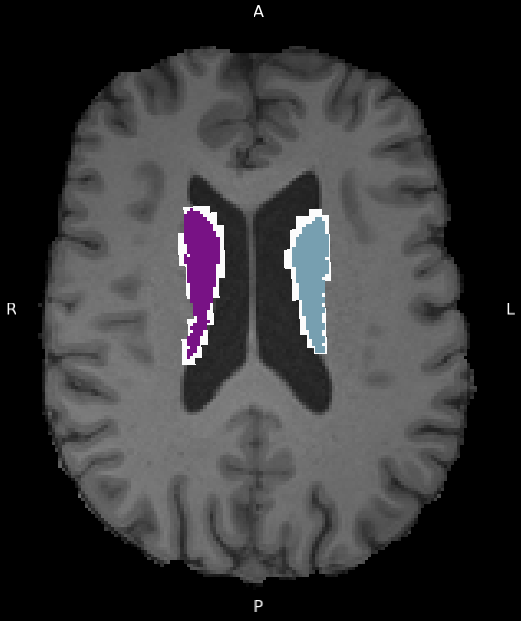
\includegraphics[width=0.3\textwidth]{basal_seg}
\caption{Basal Ganglia Subcortical Segmentation}
\label{fig:basal_seg}
\end{figure}

The figure above visualizes the alignment of the Caudate subcortical region, where the white (larger) region is the Basal Ganglia mask from the diffusion space and the colored (smaller) regions are the Basal Ganglia segmentation from T1 space.\par

In order to keep the data consistent, mapping the segmentation to the Basal Ganglia mask can be done by assigning the same label for each voxel in the basal ganglia as the label of the closest voxel in the subcortical segmentation.

\subsubsection{N-Dim Array}
The used \ac{NIfTI} format stores the raw voxel space and the affine transformation matrix separately, in order to not loose data in the process of interpolating voxels when applying the transformation. But in order to consistently compare voxel data across different spaces (even if they are registered in the same space), the transformation needs to be applied, computing the interpolated voxels in the common space, bringing them into the same raw format of matching X, Y and Z dimensions, and discarding the stored affine matrices.\par

By default the native anatomical space's origin is near the center of mass of the brain, between the ears. The makes sense for medical professionals, when working with \ac{MRI} records, but datastructure wise an array is indexed from 0. Meaning after applying the transformation to the voxel space, the yielded array will only contain one quadrant of the record as the rest are clipped in the negative regions. Thus the space is also needed to be translated with the negative vector of the transformed space's bounding box's lower end.\par

The translation value can be calculated by calculating the boundaries of the transformed space's bounding box. Get all 8 corners of the voxel space and apply the transformation matrix to all of them. Then get the min-max coordinates along X, Y and Z from the 8 transformed vectors, yielding the lower and upper bounds of the transformed space's bounding box.\par

It is very important to use the same translation value across different spaces to properly align them in the native space. For example let $D$ and $T$ denote a diffusion and t1 records and $M_D$ and $M_T$ denote their respective transformation matrices. Let $T_D$ and $T_T$ denote their respective translation values. In order to properly align them we need to apply $A_D = (M_D \cdot {\color{red}T_D})$ matrix and $A_T = (M_T \cdot {\color{red}T_D})$ matrix to $D$ and $T$ respectively, with matching ${\color{red}T_D}$ translation values.\par

The last issue is the missaligned length of the dimensions of the T1 and diffusion records. This can be simply fixed by truncating the excess along each dimension.

\subsubsection{Uniform Shape}
After aligning the data into the same space per datapoint, it is still very likely that the individual datapoints do not have a uniform shape. This is due to them being in native space, some records will contain a smaller volume brain, some will contain a larger, they will not be the same.\par
Fixing this can be done by figuring out the min-max boundaries along each axis that the brain masks take up in the voxel space. Then the range of the masks along each axis can be calculated from the lower and upper boundaries per datapoint. And then the max range can be selected per axis, across all datapoints, yielding the new uniform shape. Finally, the voxel spaces can be sliced down to the new uniform shape, which can fit all brains of all data points (with some padding for most of them).\par
Note that this fix also greatly improves space efficiency, as it cuts out the unused voxels. This will be beneficial for storage and computational demands of future experiments.
\begin{table}[H]
\centering
\begin{tabular}{|l|l|c|c|}
\hline
\textbf{Data} & \textbf{Volumes} & \textbf{Range} & \textbf{Type} \\ \hline
diffusion & 74 & $[0,4096]$ & float16 \\ \hline
diffusion\_fa & 1 & $[0,2]$ & float16 \\ \hline
diffusion\_md & 1 & $[0,0.01]$ & float16 \\ \hline
diffusion\_rd & 1 & $[0,0.01]$ & float16 \\ \hline
t1 & 1 & $[0,1000]$ & float16 \\ \hline
t1t1 & 1 & $[0,1]$ & float16 \\ \hline
targets & 14 & $\{0,1\}$ & bool \\ \hline
connectivity & 14 & $[0,1]$ & float16 \\ \hline
streamline & 14 & $[0,5000]$ & float16 \\ \hline
mask\_basal & 2 & $\{0,1\}$ & bool \\ \hline
mask\_brain & 1 & $\{0,1\}$ & bool \\ \hline
basal\_seg & 6 & $\{0,1\}$ & bool \\ \hline
\end{tabular}
\caption{Uniform Data}
\label{tab:datas2}
\end{table}
The uniform voxel space shapes are $(155,199,158)$ and $(147,191,155)$ for the native and normalized sets.

\subsection{Quality Control}

Having a low count of datapoints means that if there are even just a few outliers, it can heavily affect the end result. Thus all data were manually inspected to make sure they are clean as possible.

\subsubsection{Mismatched Data}

Looking through the diffusion, diffusion\_fa, diffusion\_md and diffusion\_rd images, 2 datapoints' \ac{FA}, \ac{MD} and \ac{RD} images were seemingly from completely different patients. Thus the \ac{FA}, \ac{MD} and \ac{RD} images were omitted for 2 datapoints.

\subsubsection{Garbled Data}

Looking through the subcortical segmentation of the Basal Ganglia revealed that 1 datapoint had a garbled segmentation. Thus, said basal\_seg image was omitted for 1 datapoint.\par
And one datapoint had a garbled T1 \ac{FNIRT} warp field. Said datapoint was entirely omitted from the normalized set of datapoints.

\subsubsection{Missing Data}

Looking through the relative connectivity and streamline images, 3 datapoints were missing these images, said 3 datapoints were completely omitted, as these datapoints are effectively missing the labels.\par
And the t1t2 images were missing for 10 datapoints, but these were not omitted as the t1 images were present for these datapoints, thus experiments only concerning the t1 can have a bit more available data.

\subsection{Radiomics Features}
Extracting the voxel based radiomic features has two main parameters to tune, the bin width and the kernel width.\par
The two approaches for binning are absolute discretization and relative discretization. Where in the prior one, a fixed bin width is chosen and in the latter one, a fixed number of bins are chosen and the bin width scales relatively according to the min-max voxel values. \citelink{bin}{This study found that "The absolute discretization consistently provided statistically significantly more reproducible features than the relative discretization."} Relying on this information, the obvious choice to start with is the absolute discretization.\par
The bin width and the kernel width will be tuned in later experiments. And possibly features calculated with different setting will be concatenated and used simultaneously for better results. The used default values will be 25 and 5 for the bin and kernel widths respectively.\par
The following types of radiomic features will be used:
\begin{table}[H]
\centering
\begin{tabular}{|l|c|}
\hline
\textbf{Feature Type} & \textbf{Number of Features} \\ \hline
first order & 18 \\ \hline
\ac{GLCM} & 23 \\ \hline
\ac{GLSZM} & 16 \\ \hline
\ac{GLRLM} & 16 \\ \hline
\ac{NGTDM} & 5 \\ \hline
\ac{GLDM} & 14 \\ \hline
3D shape & 17 \\ \hline
\end{tabular}
\caption{Radiomic Feature Types}
\label{tab:radf0}
\end{table}

\subsubsection{Voxel Based}
The following 92 features will be calculated voxel based:
\bgroup
\setlength\LTleft{-1cm}
\setlength\LTright{-1cm}
\begin{longtable}[H]{|l|l|l|}
\nobreakhline
\textbf{First Order} & \textbf{\ac{GLCM}} & \textbf{\ac{GLSZM}} \\ \nobreakhline
Energy & Autocorrelation & SmallAreaEmphasis \\ \nobreakhline
TotalEnergy & JointAverage & LargeAreaEmphasis \\ \nobreakhline
Entropy & ClusterProminence & GrayLevelNonUniformity \\ \nobreakhline
Minimum & ClusterShade & GrayLevelNonUniformityNormalized \\ \nobreakhline
10Percentile & ClusterTendency & SizeZoneNonUniformity \\ \nobreakhline
90Percentile & Contrast & SizeZoneNonUniformityNormalized \\ \nobreakhline
Maximum & Correlation & ZonePercentage \\ \nobreakhline
Mean & DifferenceAverage & GrayLevelVariance \\ \nobreakhline
Median & DifferenceEntropy & ZoneVariance \\ \nobreakhline
InterquartileRange & DifferenceVariance & ZoneEntropy \\ \nobreakhline
Range & JointEnergy & LowGrayLevelZoneEmphasis \\ \nobreakhline
MeanAbsoluteDeviation & JointEntropy & HighGrayLevelZoneEmphasis \\ \nobreakhline
RobustMeanAbsoluteDeviation & Imc1 & SmallAreaLowGrayLevelEmphasis \\ \nobreakhline
RootMeanSquared & Imc2 & SmallAreaHighGrayLevelEmphasis \\ \hline
Skewness & Idm & LargeAreaLowGrayLevelEmphasis \\ \nobreakhline
Kurtosis & MCC & LargeAreaHighGrayLevelEmphasis \\ \nobreakhline
Variance & Idmn &  \\ \nobreakhline
Uniformity & Id &  \\ \nobreakhline
 & Idn &  \\ \nobreakhline
 & InverseVariance &  \\ \nobreakhline
 & MaximumProbability &  \\ \nobreakhline
 & SumEntropy &  \\ \nobreakhline
 & SumSquares &  \\ \hline \hline
\textbf{\ac{GLRLM}} & \textbf{\ac{NGTDM}} & \textbf{\ac{GLDM}} \\ \nobreakhline
ShortRunEmphasis & Coarseness & SmallDependenceEmphasis \\ \nobreakhline
LongRunEmphasis & Contrast & LargeDependenceEmphasis \\ \nobreakhline
GrayLevelNonUniformity & Busyness & GrayLevelNonUniformity \\ \nobreakhline
GrayLevelNonUniformityNormalized & Complexity & DependenceNonUniformity \\ \nobreakhline
RunLengthNonUniformity & Strength & DependenceNonUniformityNormalized \\ \nobreakhline
RunLengthNonUniformityNormalized &  & GrayLevelVariance \\ \nobreakhline
RunPercentage &  & DependenceVariance \\ \nobreakhline
GrayLevelVariance &  & DependenceEntropy \\ \nobreakhline
RunVariance &  & LowGrayLevelEmphasis \\ \nobreakhline
RunEntropy &  & HighGrayLevelEmphasis \\ \nobreakhline
LowGrayLevelRunEmphasis &  & SmallDependenceLowGrayLevelEmphasis \\ \nobreakhline
HighGrayLevelRunEmphasis &  & SmallDependenceHighGrayLevelEmphasis \\ \nobreakhline
ShortRunLowGrayLevelEmphasis &  & LargeDependenceLowGrayLevelEmphasis \\ \nobreakhline
ShortRunHighGrayLevelEmphasis &  & LargeDependenceHighGrayLevelEmphasis \\ \nobreakhline
LongRunLowGrayLevelEmphasis &  &  \\ \nobreakhline
LongRunHighGrayLevelEmphasis &  &  \\ \nobreakhline
\caption{Voxel Based Radiomic Features}
\label{tab:radf1}
\end{longtable}
\egroup

\subsubsection{Non-Voxel Based}

\begin{table}[H]
\centering
\begin{tabular}{|l|}
\hline
\textbf{3D Shape} \\ \hline
MeshVolume \\ \hline
VoxelVolume \\ \hline
SurfaceArea \\ \hline
SurfaceVolumeRatio \\ \hline
Sphericity \\ \hline
Maximum3DDiameter \\ \hline
Maximum2DDiameterSlice \\ \hline
Maximum2DDiameterColumn \\ \hline
Maximum2DDiameterRow \\ \hline
MajorAxisLength \\ \hline
MinorAxisLength \\ \hline
LeastAxisLength \\ \hline
Elongation \\ \hline
Flatness \\ \hline
\end{tabular}
\caption{Shape Based Radiomic Features}
\label{tab:radf2}
\end{table}

